%%%%%%%%%%%%%%%%%%%%%%%%%%%%%%%%%%%%%%%%%%%%%%%%%%%%%%%%%%%%%%%%%%%%%%%%%%%%%%%%%%%%%%%%%%%%%%%%%%%%
% Project Requirements Specification Report
% Authors: Michael Galliers and James Miller
% Course: CSC 440
%%%%%%%%%%%%%%%%%%%%%%%%%%%%%%%%%%%%%%%%%%%%%%%%%%%%%%%%%%%%%%%%%%%%%%%%%%%%%%%%%%%%%%%%%%%%%%%%%%%%

\documentclass[12pt]{article}
\usepackage[utf8]{inputenc}
\usepackage{graphicx}
\usepackage{float}
\usepackage{tocloft}

% Document configuration

% Section numbering
\renewcommand \thesection{\Roman{section}}
\renewcommand \thesubsection{\arabic{section}.\arabic{subsection}}

% Environment config for requirements
%  - Configures formatting of the section heading and numbered, nested lists
\newenvironment{requirement}[1]
{
    % Format requirement sections (R1. ...)
    \renewcommand{\thesubsubsection}{R\arabic{subsubsection}.}
    % Format nested, numbered lists (1.1, 1.1.1, 1.1.1.1, ...)
    \renewcommand{\labelenumi}{
        \arabic{subsubsection}.\arabic{enumi}
    }
    \renewcommand{\labelenumii}{
        \arabic{subsubsection}.\arabic{enumi}.\arabic{enumii}
    }
    \renewcommand{\labelenumiii}{
        \arabic{subsubsection}.\arabic{enumi}.\arabic{enumii}.\arabic{enumiii}
    }
    \renewcommand{\labelenumiv}{
        \arabic{subsubsection}.\arabic{enumi}.\arabic{enumii}.\arabic{enumiii}.\arabic{enumiv}
    }
    % Create the subsubsection for the requirement
    \subsubsection{#1}
}
{}


% Set path to all graphics
\graphicspath{{figures/}}

% Do paragraph indenting after section tags
\usepackage{indentfirst}

% Adjust space between numbers and headings in table of contents
\addtolength{\cftsecnumwidth}{12pt}
\addtolength{\cftsubsubsecnumwidth}{-10pt}


\author{Michael Galliers and James Miller}
\title{CSC 440 - Requirements Specification Report}


\begin{document}

\begin{titlepage}
\maketitle
\end{titlepage}

\newpage
    \tableofcontents
\newpage

\section{Introduction}
\subsection{Problem Statement}
Chang’s Pizza is a local pizza startup. The business is in need of a way to manage orders and stock
in a systematic manor to increase revenue and workplace productivity. Currently, remote orders can
only be placed over telephone and stock management is done manually on paper. Customers have
complained about receiving incorrect orders due to employee error when transcribing orders placed
over telephone. In addition, the store has periodically run out of stock due to miscommunication
over their paper-based stock tracking system.


The idea for this project arose from personal experience, not being able to effectively manage
grades from various courses on BlackBoard. This can be due to professors not using BlackBoard to
distribute grades or the inability of BlackBoard to correctly aggregate student grades because of
an odd grading policy. This makes it difficult for students to track how well they are doing in a
course overall. As a result, students can be more or less likely to study hard for assignments,
since they believe they are doing worse or better in the course than they potentially are.

For those who decide to manage their grades themselves with pen and paper, they are able to gain
further insight into their performance in courses, but are limited by the amount of time it takes to
manage and compute statistics about their grades. As a student, there should be a simple way to
manage and visualize grades, without the need to do calculations by hand.


As EKU college students, we (the authors) have firsthand experience with the difficulties of
grade/progress management. The tools already used by the college for grade management have their
flaws. Many professors either do not setup the grade configuration properly (designation of
categories and weights), or they choose to not use BlackBoard for tracking grades at all. Also,
BlackBoard does not have the ability to give insights on students grades other than simple weighted
averages or totals.

For those students who decide to manage grades by hand themselves, they are able to
gain further insight into their performance in courses, but are limited by the amount of time it
takes to do manual computations on those grades. As a student, there should be a simple way to manage
grades and course progress and visualize grades, without the need to do calculations by hand.


First, the grade tracking feature of BlackBoard is not a central feature to the service.
Thus, the feedback on a students score 
\subsection{Proposal}

\section{System Description}

\section{System Requirements}
\subsection{Functional Requirements}
\begin{requirement}{The system shall..1}


\begin{enumerate}
    \item Test item 1
    \item Test item 2
    \begin{enumerate}
        \item Test item 1.1
        \item Test item 1.2
        \begin{enumerate}
            \item Test item 1.1.1
            \item Test item 1.1.2
            \begin{enumerate}
                \item Test item 1.1.1.1
                \item Test item 1.1.1.2
            \end{enumerate}
        \end{enumerate}
    \end{enumerate}
\end{enumerate}


\end{requirement}

\begin{requirement}{The system shall..2}


\begin{enumerate}
    \item Test item 1
    \item Test item 2
    \begin{enumerate}
        \item Test item 1.1
        \item Test item 1.2
        \begin{enumerate}
            \item Test item 1.1.1
            \item Test item 1.1.2
            \begin{enumerate}
                \item Test item 1.1.1.1
                \item Test item 1.1.1.2
            \end{enumerate}
        \end{enumerate}
    \end{enumerate}
\end{enumerate}


\end{requirement}

\subsection{Non-functional Requirements}

\subsection{Domain Requirements}

\section{Use-case Diagram}

\section{Class Diagram}

\section{Sequence Diagrams}

\section{State Diagram}

\section{Activity Diagrams}

\section{Database Design}

\begin{figure}[p!]
  \subsection{ER Schema}
  \centering
  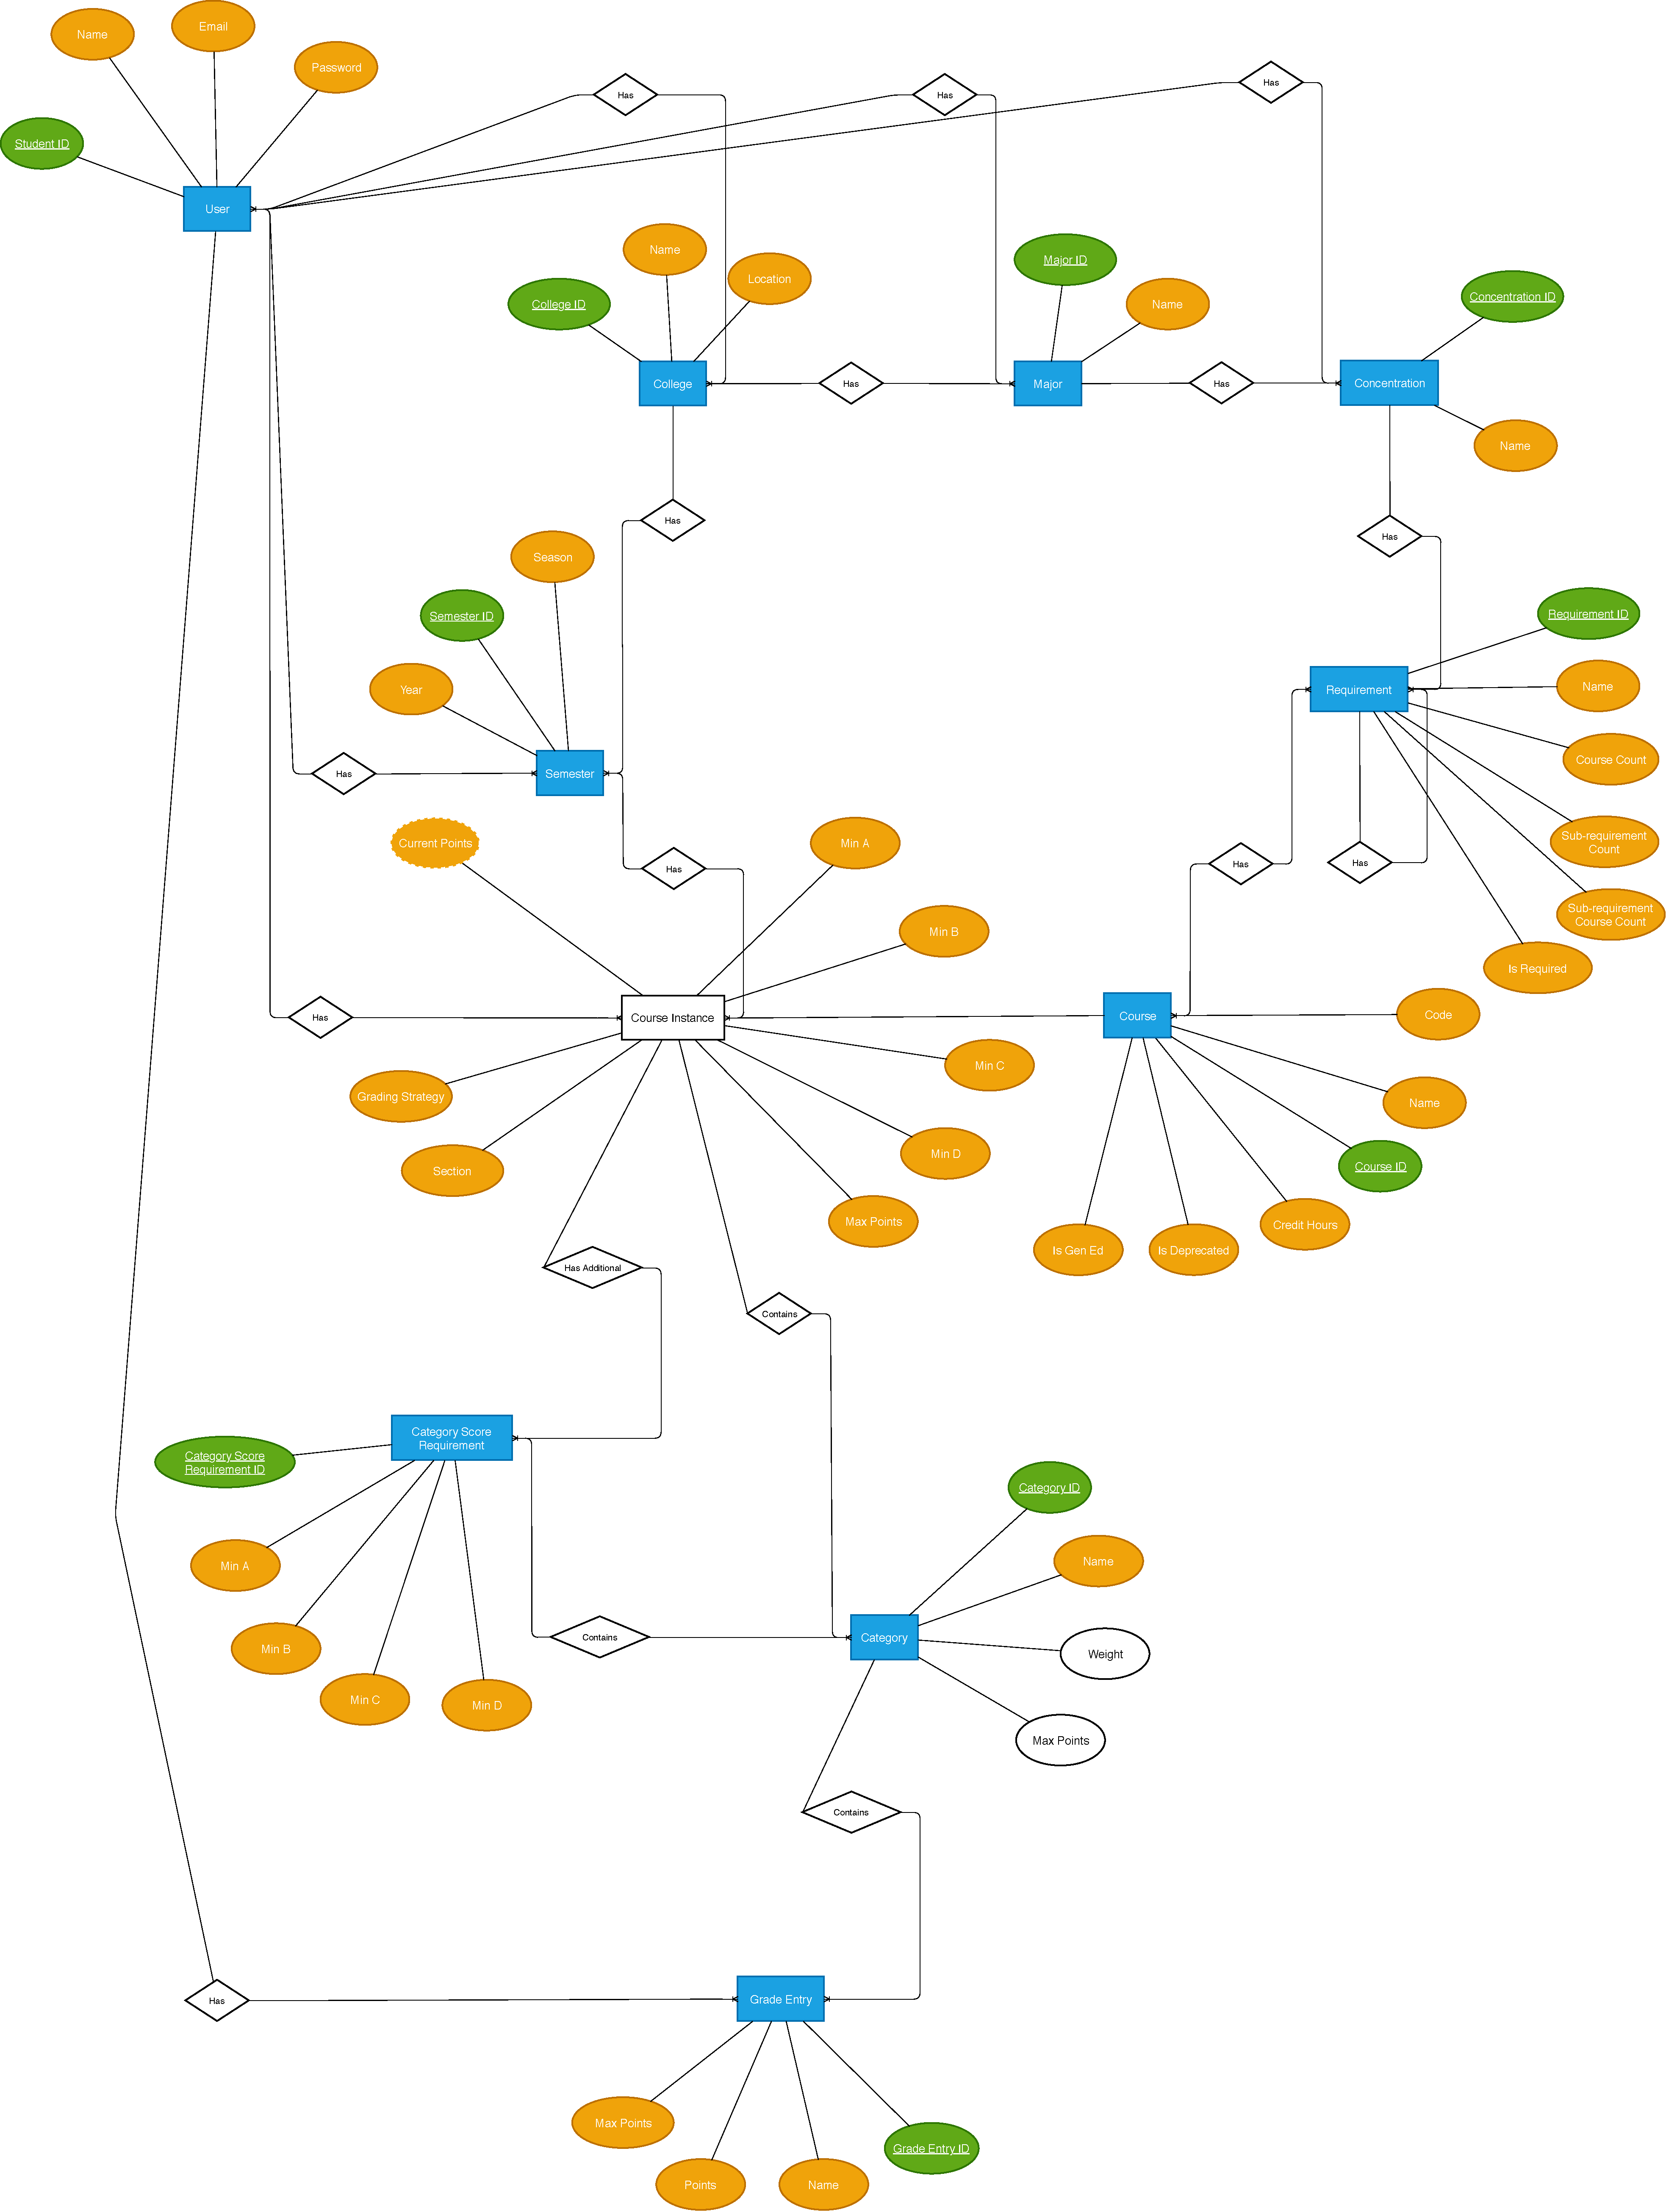
\includegraphics[width=\linewidth]{database_erd.pdf}
  \caption{Database ERD}
\end{figure}

\clearpage

\subsection{Table Schema}

\section{Conclusion}

\section{Dictionary}
\begin{itemize}
    \item \textbf{Semester}: A single semester of education consisting of courses. Each semester can
    be associated with a different educational institution; consistency is not required.
    \item \textbf{Course}: Any educational course/class occurring within a particular semester.
    \item \textbf{Section}: An equally weighted or logically grouped collection of material within a
    particular course (e.g. Homework, Tests, etc.).
    \item \textbf{Grade Entry}: A graded piece of material associated with a particular section 
    (e.g. Homework 2, Exam 1, etc.).
\end{itemize}

\end{document}
